ND-Range和分层并行内核将工作项组织到工作组中,并且工作组中的工作项可以并发执行。工作项可以保证并发时,工作组中的中的协作问题才能解决。\par

\hspace*{\fill} \par %插入空行
图9-1 二维ND-Range中(8,8)个工作项分为四个(4,4)工作组
\begin{center}
	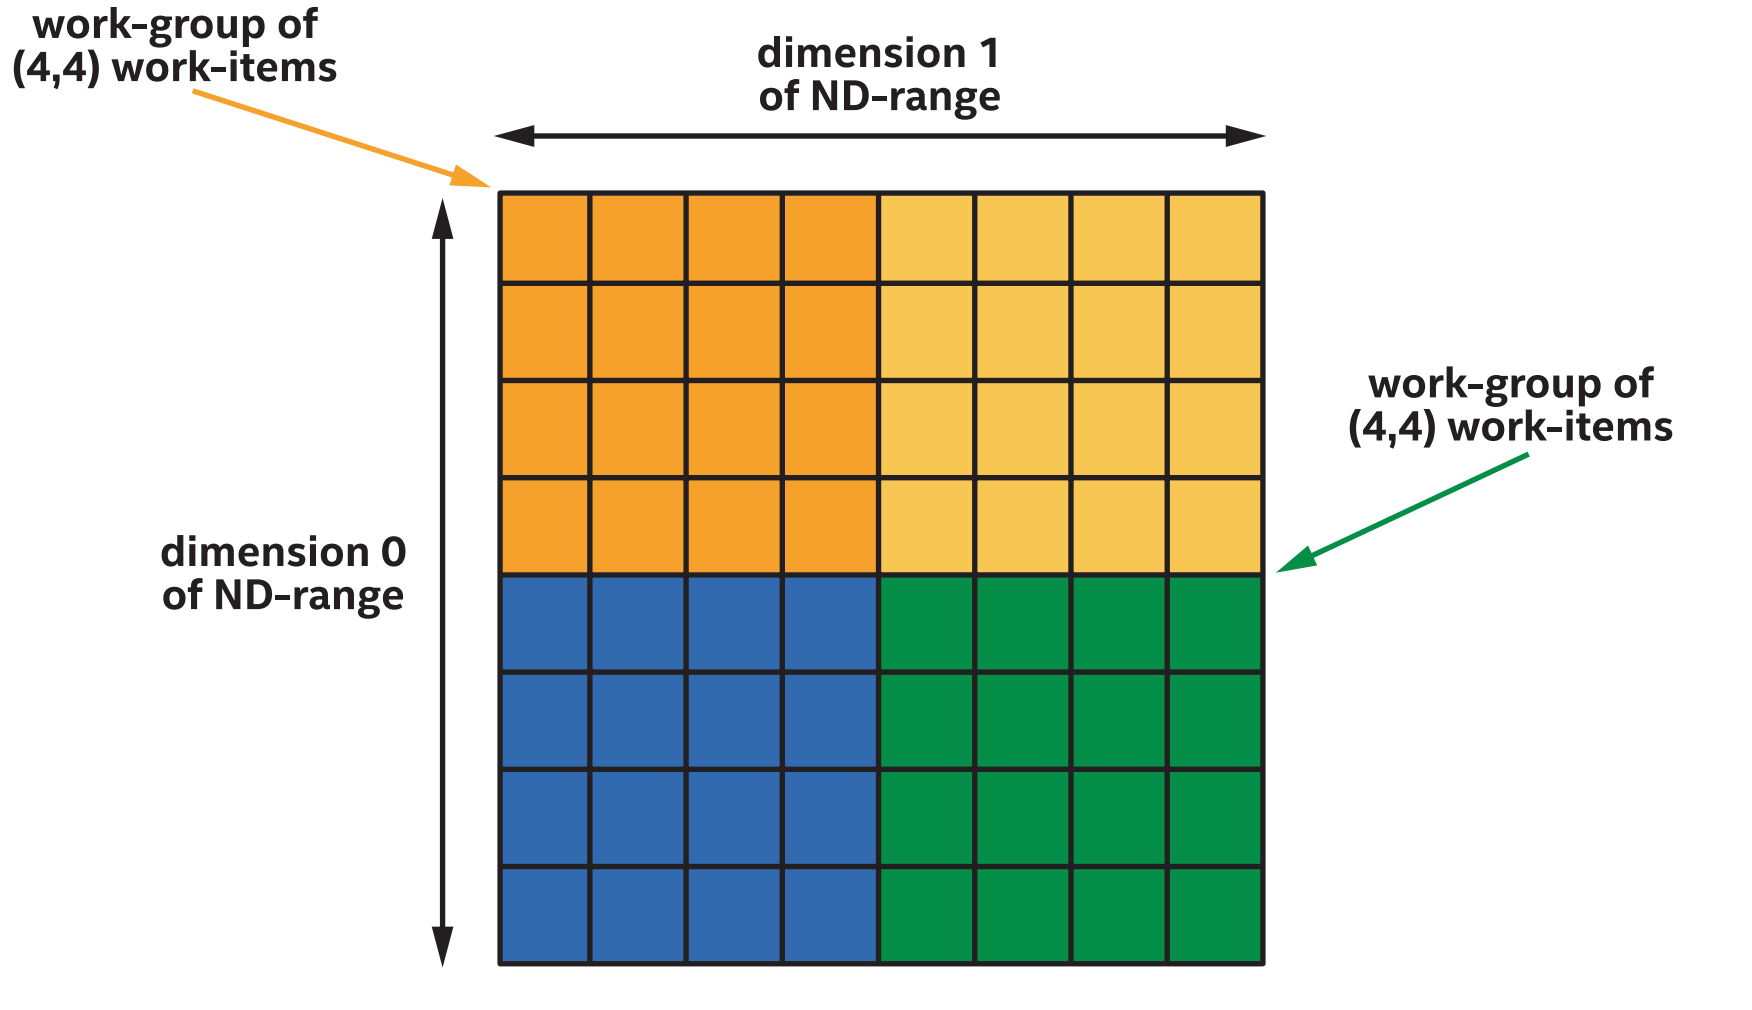
\includegraphics[width=1.\textwidth]{content/chapter-9/images/2}
\end{center}

图9-1将ND-Range划分为不同的工作组,每个工作组用不同的颜色表示。工作组中的工作项可以同时执行,因此工作项可以与相同颜色的工作项通信。\par

因为不同工作组不能保证并发执行,所以同一种颜色的工作项不能与不同颜色的工作项通信,并且如果一个工作项试图与当前未执行的另一个工作项通信,可能会导致死锁。当我们希望内核完成执行,必须确保当工作项之间通信时,必须在同一个工作组中。\par















































